%% ****** Start of file apstemplate.tex ****** %
%%
%%
%%   This file is part of the APS files in the REVTeX 4 distribution.
%%   Version 4.1r of REVTeX, August 2010
%%
%%
%%   Copyright (c) 2001, 2009, 2010 The American Physical Society.
%%
%%   See the REVTeX 4 README file for restrictions and more information.
%%
%
% This is a template for producing manuscripts for use with REVTEX 4.0
% Copy this file to another name and then work on that file.
% That way, you always have this original template file to use.
%
% Group addresses by affiliation; use superscriptaddress for long
% author lists, or if there are many overlapping affiliations.
% For Phys. Rev. appearance, change preprint to twocolumn.
% Choose pra, prb, prc, prd, pre, prl, prstab, prstper, or rmp for journal
%  Add 'draft' option to mark overfull boxes with black boxes
%  Add 'showpacs' option to make PACS codes appear
%  Add 'showkeys' option to make keywords appear
\documentclass[aps,twocolumn,secnumarabic,amsmath,amssymb,pra,groupedaddress,
showpacs, showkeys]{revtex4-1}
%\documentclass[aps,prl,preprint,superscriptaddress]{revtex4-1}
%\documentclass[aps,prl,reprint,groupedaddress]{revtex4-1}

% You should use BibTeX and apsrev.bst for references
% Choosing a journal automatically selects the correct APS
% BibTeX style file (bst file), so only uncomment the line
% below if necessary.
%\bibliographystyle{apsrev4-1}

\usepackage{color}         % produces boxes or entire pages with colored backgrounds
\usepackage{graphics}      % standard graphics specifications
\usepackage[pdftex]{graphicx}      % alternative graphics specifications
\usepackage{longtable}     % helps with long table options
\usepackage{epsf}          % old package handles encapsulated post script issues
\usepackage{bm}            % special 'bold-math' package
\usepackage{thumbpdf}
\usepackage[colorlinks=true]{hyperref}  % this package should be added after all others
                                        % use as follows: \url{http://web.mit.edu/8.13}
\usepackage{verbatim}
\usepackage{subfigure}


\newcommand{\sech}{\mathop{\rm sech}\nolimits}
\newcommand{\bra}[1]{\left\langle #1 \right|}
\newcommand{\ket}[1]{\left|#1\right\rangle}
\newcommand{\braket}[2]{\left\langle#1 |  #2\right\rangle}
\newcommand{\rd}[1]{\mathop{\mathrm{d}#1}}
\newcommand{\ad}{\mathop{\hat{a}^{\dagger}}}
\newcommand{\bd}{\mathop{\hat{b}^{\dagger}}}
\newcommand{\cda}{\mathop{\hat{c}_+^{\dagger}}}
\newcommand{\cds}{\mathop{\hat{c}_-^{\dagger}}}
\newcommand{\parena}[1]{\left(#1\right)}
\newcommand{\parenb}[1]{\left[#1\right]}
\newcommand{\pna}[1]{\left(#1\right)}
\newcommand{\pnb}[1]{\left[#1\right]}
\newcommand{\eqn}[1]{
\begin{equation}
	#1
\end{equation}
}
\newcommand{\avg}[1]{\langle\langle #1 \rangle\rangle}
\newcommand{\avga}[1]{\langle #1 \rangle}
\newcommand{\mcl}[1]{\mathcal{#1}}
\newcommand{\soln}[1]{\textcolor{blue}{#1}}
\newcommand{\abs}[1]{\left|#1\right|}

\begin{document}

% Use the \preprint command to place your local institutional report
% number in the upper righthand corner of the title page in preprint mode.
% Multiple \preprint commands are allowed.
% Use the 'preprintnumbers' class option to override journal defaults
% to display numbers if necessary
%\preprint{}

%Title of paper
\title{Polarization Entanglement Distribution in Ensemble-Based Atomic Memories}

% repeat the \author .. \affiliation  etc. as needed
% \email, \thanks, \homepage, \altaffiliation all apply to the current
% author. Explanatory text should go in the []'s, actual e-mail
% address or url should go in the {}'s for \email and \homepage.
% Please use the appropriate macro foreach each type of information

% \affiliation command applies to all authors since the last
% \affiliation command. The \affiliation command should follow the
% other information
% \affiliation can be followed by \email, \homepage, \thanks as well.

\author{Bhaskar Mookerji}
\email{mookerji@mit.edu}
\affiliation{Massachusetts Institute of Technology, Cambridge, Massachusetts 02139, USA}
\author{Jeffrey H. Shapiro}
\email{jhs@mit.edu}
\affiliation{Massachusetts Institute of Technology, Research Laboratory of Electronics, Cambridge, Massachusetts 02139, USA}

%Collaboration name if desired (requires use of superscriptaddress
%option in \documentclass). \noaffiliation is required (may also be
%used with the \author command).
%\collaboration can be followed by \email, \homepage, \thanks as well.
%\collaboration{}
%\noaffiliation

\date{\today}

\begin{abstract}

  Quantum networks enable the long-distance communication of quantum states
  through teleportation, but require, in advance, the robust distribution of
  entanglement between relevant parties. Engineering these networks requires
  quantum interconnects, which convert quantum states in one physical system to
  those of another reversibly, and with high fidelity. In the following, we
  describe implementations of long-distance quantum communication networks
  using polarization entanglement and atomic ensembles. We concisely describe
  the interactions of a quantum optical field with a heralding atomic ensemble,
  accounting for multiple-pair events at entanglement generation, as well as
  finite transmission and photodetection efficiencies under number-resolving
  and non-resolving photodetection schemes. Using these results, we perform a
  detailed quantitative performance analysis of quantum networks that
  distribute and swap entanglement.

\end{abstract}

% insert suggested PACS numbers in braces on next line
\pacs{}
% insert suggested keywords - APS authors don't need to do this
%\keywords{}

%\maketitle must follow title, authors, abstract, \pacs, and \keywords
\maketitle

% body of paper here - Use proper section commands
% References should be done using the \cite, \ref, and \label commands
\section{}
% Put \label in argument of \section for cross-referencing
%\section{\label{}}
\subsection{}
\subsubsection{}

% If in two-column mode, this environment will change to single-column
% format so that long equations can be displayed. Use
% sparingly.
%\begin{widetext}
% put long equation here
%\end{widetext}

% figures should be put into the text as floats.
% Use the graphics or graphicx packages (distributed with LaTeX2e)
% and the \includegraphics macro defined in those packages.
% See the LaTeX Graphics Companion by Michel Goosens, Sebastian Rahtz,
% and Frank Mittelbach for instance.
%
% Here is an example of the general form of a figure:
% Fill in the caption in the braces of the \caption{} command. Put the label
% that you will use with \ref{} command in the braces of the \label{} command.
% Use the figure* environment if the figure should span across the
% entire page. There is no need to do explicit centering.

% \begin{figure}
% \includegraphics{}%
% \caption{\label{}}
% \end{figure}

% Surround figure environment with turnpage environment for landscape
% figure
% \begin{turnpage}
% \begin{figure}
% \includegraphics{}%
% \caption{\label{}}
% \end{figure}
% \end{turnpage}

% tables should appear as floats within the text
%
% Here is an example of the general form of a table:
% Fill in the caption in the braces of the \caption{} command. Put the label
% that you will use with \ref{} command in the braces of the \label{} command.
% Insert the column specifiers (l, r, c, d, etc.) in the empty braces of the
% \begin{tabular}{} command.
% The ruledtabular enviroment adds doubled rules to table and sets a
% reasonable default table settings.
% Use the table* environment to get a full-width table in two-column
% Add \usepackage{longtable} and the longtable (or longtable*}
% environment for nicely formatted long tables. Or use the the [H]
% placement option to break a long table (with less control than 
% in longtable).
% \begin{table}%[H] add [H] placement to break table across pages
% \caption{\label{}}
% \begin{ruledtabular}
% \begin{tabular}{}
% Lines of table here ending with \\
% \end{tabular}
% \end{ruledtabular}
% \end{table}

% Surround table environment with turnpage environment for landscape
% table
% \begin{turnpage}
% \begin{table}
% \caption{\label{}}
% \begin{ruledtabular}
% \begin{tabular}{}
% \end{tabular}
% \end{ruledtabular}
% \end{table}
% \end{turnpage}

%% This is an example first chapter.  You should put chapter/appendix that you
%% write into a separate file, and add a line \include{yourfilename} to
%% main.tex, where `yourfilename.tex' is the name of the chapter/appendix file.
%% You can process specific files by typing their names in at the 
%% \files=
%% prompt when you run the file main.tex through LaTeX.

\section{Heralded Polarization Entanglement Distribution with Atomic
  Ensembles\label{chap:herald}}

This chapter combines the operating principles of ensemble-based quantum
memories, as described in Chapter~\ref{chap:atomic}, with architectures for
polarization entanglement distribution, entanglement connection, and quantum
teleportation. We will first discuss our architecture for entanglement
distribution and provide a very basic abstraction for quantum memories. The
remainder characterizes figures of merit---fidelity, heralding probability, and
protocol success probability---under various transmission loss and
photodetection conditions.

\subsection{Architecture Overview and Figures of Merit\label{sec:herald:overview}}

\begin{figure*}[t]
	\centering
	\resizebox{6.50in}{!}{\input spdc_dlcz_fin.pdf_t}
	\caption{Modified DLCZ architecture for distributing polarization entanglement, using a spontaneous parametric downconversion (SPDC) source and  interferometer measurement for entanglement verification.}
	\label{fig:channel_model}
\end{figure*}

\begin{figure*}[htb]
	\centering
	\resizebox{6.50in}{!}{\input spdc_dlcz_loss.pdf_t}
	\caption{Hong-Ou-Mandel (HOM) interferometer measurement with loss (labeled).}
	\label{fig:channel_loss_model}
\end{figure*}

We will first discuss our overall architecture and loss model, followed by
particular details of a dual-OPA polarization entanglement source and quantum
memories. Our architecture for polarization entanglement distribution, shown in
Fig.~\ref{fig:channel_model}, is a modification of the standard DLCZ
architecture shown in Fig.~\ref{fig:dlcz}. In the original DLCZ protocol, both
ensembles are coherently pumped and the probability that both ensembles will
emit single photons is low compared to that for emission from a single
ensemble. Interference at the 50-50 beam splitter in Fig.~\ref{fig:dlcz} erases
any which-path information for the emission event, so a single detection at
either photon counter $D_1$ or $D_2$ is used to herald entanglement of the two
ensembles. The ideal situation in Fig.~\ref{fig:channel_model} is when a
polarization singlet is emitted from the source and the overall system is
lossless. The polarizing beam splitters (PBS) then load the signal and idler
photons from the singlet into a coherent superposition of excitations of
ensembles 1 and 2 and ensembles 3 and 4, respectively. This loading is heralded
by the single-photon detections from pair $\pna{D_1, D_2}$ and $\pna{D_3,
  D_4}$.

Fig.~\ref{fig:channel_loss_model} encompasses the error modes for the
Fig.~\ref{fig:channel_model} distribution architecture. The Type-II SPDC source
may produce multiple signal-idler pairs, which will be modeled with the full
joint Gaussian state description of its output. Propagation losses between the
PBS and the atomic ensembles (labelled `pre'), and between the atomic ensembles
and the 50-50 beam splitter (labelled `post') are modeled by fictitious beam
splitters whose vacuum-state input ports inject Gaussian quantum noise. Finite
quantum efficiency photodetectors (labelled `pho') are similarly modeled, and
we have ignored dark counts, which are known to be reasonably low at heralding
wavelengths for silicon Geiger-mode avalanche photodiodes
(APDs)~\cite{Thomas2010}. Our number state model for these fictitious beam
splitters, described in Section~\ref{sec:herald:number}, includes the effects
of phase differences between input ports, which we can use to characterize the
effects of phase mismatch between pairs of ensembles. We will assume that any
accumulated phase offsets leading to the ensembles can be incorporated into the
pre-transmission efficiency.

The preceding imperfections expose two fundamentally different failure modes
for this protocol that affect fidelity and probability of success,
respectively. First, is it possible for heralding detections at the APDs to
declare the protocol's success even when the ensembles themselves are not in a
polarization singlet state. For example, a multiple-pair event from the
entanglement source could lead to multiple heralding photons emitted by a
quantum memory. Post-memory attenuation and finite-quantum efficiency
photodetection could eliminate all but one of those heralding photons, and the
usage of Geiger-mode APDs might completely preclude our ability to distinguish
between multiple-photon and single-photon events. A relative phase offset
between two ensembles, either because of pump photon phase mismatch or
pre-transmission phase accumulation, would similarly affect the final fidelity
of the loaded quantum state. Lastly, because post-memory imperfections reduce
potential heralding detections, it possible to declare the protocol a
failure---and reduce the probability of success---even when the ensembles are
successfully loaded.

We characterize this architecture's performance of heralding entanglement
distribution by determining its fidelity figure-of-merit and measurement
statistics under different photodetection schemes: photon-number resolving
detection (PNRD), which can distinguish between single-photon and multi-photon
photodetection events; and non-resolving single-photon detection (NRPD), which
is unable to exclude multi-photon error events. For these two schemes, the
projective measurement operators $\hat{M}_j~\pna{j=1,2,3,4}$ represent four
successful heralding outcomes at the photodetectors $D_i~\pna{i=1,2,3,4}$. The
input to each 50-50 beam splitter in Fig.~\ref{fig:channel_model} is a
superposition state of linearly co-polarized heralding photons from the atomic
memories, so we expect that successful entanglement distribution to yield
single clicks at the signal and idler photodetector pairs. This DLCZ-like
protocol for heralded polarization entanglement distribution therefore requires
the occurrence of a single detection on either photodetectors $D_1$ or $D_2$,
as well as a \emph{corresponding event} on either $D_4$ or $D_3$. In the
following, successful heralding is given by the projective measurements
\begin{align}
    \hat{M}_j^{\textrm{PNRD}} = \left\{
	\begin{array}{lr}
\pna{\ket{1}_{11}\bra{1}}\otimes\pna{\ket{0}_{22}\bra{0}}\otimes\pna{\ket{1}_{33}\bra{1}}\otimes\pna{\ket{0}_{44}\bra{0}} & j=1\\
\pna{\ket{0}_{11}\bra{0}}\otimes\pna{\ket{1}_{22}\bra{1}}\otimes\pna{\ket{1}_{33}\bra{1}}\otimes\pna{\ket{0}_{44}\bra{0}} & j=2\\
\pna{\ket{0}_{11}\bra{0}}\otimes\pna{\ket{1}_{22}\bra{1}}\otimes\pna{\ket{0}_{33}\bra{0}}\otimes\pna{\ket{1}_{44}\bra{1}} & j=3\\
\pna{\ket{1}_{11}\bra{1}}\otimes\pna{\ket{0}_{22}\bra{0}}\otimes\pna{\ket{0}_{33}\bra{0}}\otimes\pna{\ket{1}_{44}\bra{1}} & j=4
	\end{array}
	\right.,
\end{align}

\begin{align}
    \hat{M}_j^{\textrm{NRPD}} = \left\{
	\begin{array}{lr}
\pna{\hat{I}_1-\ket{0}_{11}\bra{0}}\otimes\pna{\ket{0}_{22}\bra{0}}\otimes\pna{\hat{I}_3-\ket{0}_{33}\bra{0}}\otimes\pna{\ket{0}_{44}\bra{0}} & j=1\\
\pna{\ket{0}_{11}\bra{0}}\otimes\pna{\hat{I}_2-\ket{0}_{22}\bra{0}}\otimes\pna{\hat{I}_3-\ket{0}_{33}\bra{0}}\otimes\pna{\ket{0}_{44}\bra{0}} & j=2\\
\pna{\ket{0}_{11}\bra{0}}\otimes\pna{\hat{I}_2-\ket{0}_{22}\bra{0}}\otimes\pna{\ket{0}_{33}\bra{0}}\otimes\pna{\hat{I}_4-\ket{0}_{44}\bra{0}} & j=3\\
\pna{\hat{I}_1-\ket{0}_{11}\bra{0}}\otimes\pna{\ket{0}_{22}\bra{0}}\otimes\pna{\ket{0}_{33}\bra{0}}\otimes\pna{\hat{I}_4-\ket{0}_{44}\bra{0}} & j=4
	\end{array}
	\right.,
	\label{eq:chap3:meas_povm}
\end{align}
where $\ket{n}_i$ ($n=0,1$) are the vacuum and single-photon states, and
$\hat{I}_i$ is the identity operator for the $\hat{a}_i$ mode measured at
photodetector $D_i$ ($i=1,2,3,4$).

The heralding probability $P_{\textrm{herald}}$ is the probability a
heralding---a $\pna{D_1, D_2}$ single slick and a $\pna{D_3, D_4}$ single
click. The success probability $P_{\textrm{success}}$ is the probability that
heralding has occurred and the four ensembles have loaded a polarization Bell
state. The fidelity $F_j$ is the projection of the post-heralding ensemble
state onto the appropriate Bell state for $\hat{M}_j$ heralding, i.e.,
\eqn{
\ket{\psi_j} = \frac{1}{\sqrt{2}}\pna{\ket{1}_S^1\ket{0}_S^2\ket{0}_S^3\ket{1}_S^4+\pna{-1}^j \ket{0}_S^1\ket{1}_S^2\ket{1}_S^3\ket{0}_S^4} \qquad \pna{j=1,2,3,4}.\label{eqn:remaining_singlet}
}
Following a photodetection measurement, the joint density operator of the four
atomic ensembles is determined by applying $\hat{M}_j$ and tracing over the
optical modes:
	\eqn{
	\hat{\rho}_{\textrm{post}}^j=\frac{1}{P_j^{\textrm{herald}}}\textrm{tr}_{1,2,3,4}\pna{\hat{\rho}_{\textrm{out}}\hat{M}_j}
	}
	where $\hat{\rho}_{\textrm{out}}$ is the joint density operator of the heralding light fields and the ensembles 
	\eqn{
	P_j^{\textrm{herald}}=\textrm{tr}\pna{\hat{\rho}_{\textrm{out}}\hat{M}_j} \label{eqn:herald_prob}.
}
If $\ket{\psi_j}$ is the entangled state of the four ensembles as heralded by
$\hat{M}_j$, and the entanglement storage fidelity is $F_j$, we find that the
success probability is
\eqn{
P_{\textrm{success}} = \sum_{j=1}^4 P_j^{\textrm{herald}} F_j =\sum_{j=1}^{4} \textrm{tr}\pna{\hat{\rho}_{\textrm{out}}\hat{M}_j} \bra{\psi_j} \hat{\rho}_{\textrm{post}}^j \ket{\psi_j}.\label{eq:success_prob_def}  
}
We will determine these measurement statistics using a full number-state
analysis. Because the successful heralding outcomes defined by $\hat{M}_j$ are
symmetric, all the fidelities $F_j$ are equal to each other. We will,
therefore, calculate only $F_1$ without any loss of generality.  In what
immediately follows, we will formalize our approach for calculating the joint
density operator of the light-ensemble system following entanglement
distribution.

\subsection{Photon Number Probability Distributions}

\begin{figure}[tb]
	\centering
	\resizebox{3.00in}{!}{\input beamsplitter.pdf_t}
	\caption{Beam splitter action on an input density operator $\hat{\rho}_{\textrm{in}}$ with two input ports and two output ports. Labeled at each port are the input and output bases used in Eqns.~\ref{eqn:chap3_rho_input} and~\ref{eqn:chap3_rho_output}. The boson annihilation operations at the input and output are $\hat{a}_i$ and $\hat{b}_i$, respectively, and the accompanying index $i$ represents signal ($i=1$) and auxiliary modes ($i=2$).}
	\label{fig:beamsplitter_model}
\end{figure}

Our first task is to concisely represent the effects of propagation loss on
light beams of arbitrary statistical composition, as shown by the unitary beam
splitter transformation in Fig.~\ref{fig:beamsplitter_model}.  The matrix
representation of linear-loss beam splitters in
Fig.~\ref{fig:channel_loss_model} corresponds to the $\textrm{SU}\pna{2}$ Lie
group representation from angular momentum
quantization~\cite{PhysRevA.40.1371}. We can use this equivalence to concisely
relate the input and output field density operators from the loss using a joint
photon-number probability distribution.

A two-port beam splitter with quantum efficiency $\eta$ and input-field phase
shifts $\phi_t$ and $\phi_r$ is described by the general $\textrm{SU}\pna{2}$
beam splitter operator,
\eqn{
\hat{B}\pna{\eta,\phi_t,\phi_r}=e^{-i\pna{\phi_t-\phi_r}\hat{L}_3}e^{-2i\cos^{-1}\pna{\sqrt{\eta}}\hat{L}_2}e^{-i\pna{\phi_t+\phi_r}\hat{L}_3},\label{eq:bs_operator_def}
}
where the $\{\hat{L}_i\}$ are the Schwinger angular momentum operators for a
two-dimensional quantum harmonic oscillator:
\eqn{
\hat{L}_1 = \frac{1}{2}\pna{\hat{a}_1^{\dagger}\hat{a}_2+\hat{a}^{\dagger}_2\hat{a}_1} \quad 
\hat{L}_2 = \frac{1}{2i}\pna{\hat{a}_1^{\dagger}\hat{a}_2-\hat{a}^{\dagger}_2\hat{a}_1}\quad 
\hat{L}_3 = \frac{1}{2}\pna{\hat{a}_1^{\dagger}\hat{a}_1+\hat{a}^{\dagger}_2\hat{a}_2}.
}
Given a joint input state---either a pure state $\ket{\psi}_{\textrm{in}}$, or
a pure or mixed state $\hat{\rho}_{\textrm{in}}$---of the signal and auxiliary
inputs, the output state of the beam splitter is
\eqn{
\ket{\psi_{\textrm{out}}}=\hat{B}^{\dagger}\pna{\eta,\phi_t,\phi_r}\ket{\psi_{\textrm{in}}}, \qquad 
\hat{\rho}_{\textrm{out}}=\hat{B}^{\dagger}\pna{\eta,\phi_t,\phi_r}\hat{\rho}_{\textrm{in}}\hat{B}\pna{\eta,\phi_t,\phi_r}.\label{eq:beamsplitter_trans}}

In the number-state representation, as shown in
Fig.~\ref{fig:beamsplitter_model}, the beam splitter output of a general joint
input state
\eqn{
\hat{\rho}_{\textrm{in}}=\sum_{n_1,n_2=0}^{\infty}\sum_{n_1',n_2'=0}^{\infty}
\rho_{\textrm{in}}\pna{n_1,n_2;n_1',n_2'}\ket{n_1,n_2}\bra{n_1',n_2'} \label{eqn:chap3_rho_input}
}
is,
\eqn{
\hat{\rho}_{\textrm{out}}=\sum_{N_1,N_2=0}^{\infty}\sum_{N_1',N_2'=0}^{\infty}
\rho_{\textrm{out}}\pna{N_1,N_2;N_1',N_2'}\ket{N_1,N_2}\bra{N_1',N_2'},\label{eqn:chap3_rho_output}.
}
The output state (Eqn.~\ref{eqn:chap3_rho_output}) follows from the input state
(Eqn.~\ref{eqn:chap3_rho_input}) by first applying the unitary beam splitter
transformation in Eqn.~\ref{eq:bs_operator_def}, and then inserting the
identity operator in the $\ket{N_1,N_2}$ basis. The output matrix elements in
Eqn.~\ref{eqn:chap3_rho_output} are
\eqn{\rho_{\textrm{out}}\pna{N_1,N_2;N_1',N_2'}=\sum_{n_1,n_2=0}\sum_{n_1',n_2'=0} B_{N_1,N_2}^{n_1,n_2}\pna{\eta,\phi_t,\phi_r}\pnb{B_{N_1',N_2'}^{n_1',n_2'}\pna{\eta,\phi_t,\phi_r}}^{*}\rho_{\textrm{in}}\pna{n_1,n_2;n_1',n_2'},\label{eq:rho_output}
}
where
\begin{align}
B_{N_1,N_2}^{n_1,n_2}\pna{\eta,\phi_t,\phi_r} &= \bra{N_1,N_2}\hat{B}^{\dagger}\pna{\eta,\phi_t,\phi_r}\ket{n_1,n_2}\nonumber \\
& =R_{N_1,N_2}^{n_1,n_2}\pna{\eta} e^{i{\phi_t\pna{N_1-n_2}+\phi_r\pna{N_1-n_1}}}.
\end{align}
The transformation coefficients,
\eqn{
R_{N_1,N_2}^{n_1,n_2}\pna{\eta}=\abs{B_{N_1,N_2}^{n_1,n_2}\pna{\eta,\phi_t,\phi_r}}=\bra{N_1,N_2}e^{-2i\cos^{-1}\pna{\sqrt{\eta}}\hat{L}_2}\ket{n_1,n_2},
}
can be calculated in terms of the Jacobi polynomials $P_n^{\pna{\alpha,\beta}}\pna{x}$ as
\begin{align}
	R_{N_1,N_2}^{n_1,n_2}\pna{\eta}=\sqrt{\frac{N_1!N_2!}{n_1!n_2!} \eta^{N_1-n_2}\pna{1-\eta}^{N_1-n_1}}P_{N_2}^{\pna{N_1-n_1,N_1-n_2}}\pna{2\eta-1}, \qquad N_1\geq n_1,n_2,  \label{eqn:coefficient_value}
\end{align}
where
\begin{align}
P_n^{\pna{\alpha,\beta}}\pna{x} = \frac{\pna{-1}^n}{2^n n!}\pna{1-x}^{-\alpha}\pna{1+x}^{-\beta}\pna{\frac{d}{dx}}^n\pnb{\pna{1-x}^{n+\alpha}\pna{1+x}^{n+\beta}},\nonumber \\
\alpha,\beta >-1, \quad -1\leq x \leq 1.
\end{align}
The restriction $N_1\geq n_1, n_2$ ensures the orthogonality of the Jacobi
polynomials in Eqn.~\ref{eqn:coefficient_value} over the range of quantum
efficiency $0\leq \eta \leq 1$; we will extend the range of this coefficient
shortly. The $R$ coefficient characterizes the output photon-number probability
distribution for the joint input state $\ket{n_1,n_2}$. For a number-diagonal
joint input state, it can be shown that
\eqn{
    P_{\textrm{out}}\pna{N_1, N_2} = \bra{N_1, N_2} \hat{\rho}_{\textrm{out}}\ket{N_1, N_2}
    = \sum_{\substack{n_1=0\\n_2=N_1+N_2-n_1}}^{N_1+N_2}P_{\textrm{out}}\pna{N_1, N_2|n_1, n_2} P_{\textrm{in}}\pna{n_1, n_2},}
where the conditional and joint probabilities are 
\eqn{
P_{\textrm{out}}\pna{N_1, N_2|n_1, n_2} = \pnb{R_{N_1,N_2}^{n_1,n_2}\pna{\eta}}^2
\quad \textrm{and} \quad 
P_{\textrm{in}}\pna{n_1, n_2} = \rho_{\textrm{in}}\pna{n_1,n_2;n_1,n_2},
} respectively.

The beam splitter's physical symmetries allow us to extend the Jacobi
polynomials over the full range photon-number output probabilities:
\eqn{
   R_{N_1,N_2}^{n_1,n_2}\pna{\eta} = \left\{
     \begin{array}{lr}
        \pna{-1}^{N_1 - n_1} R_{n_1,n_2}^{N_1,N_2}\pna{\eta} & n_2 \leq N_1 < n_1 \\
       R_{n_2,n_1}^{N_2,N_1}\pna{\eta} & n_1 \leq N_1 < n_2 \\
	   \pna{-1}^{N_1 - n_1} R_{N_2,N_1}^{n_2,n_1}\pna{\eta} &\qquad n_1 > N_1,~n_2 > N_1 \\
	0 & n_1+n_2\neq N_1+N_2
     \end{array}
\right..}
We have made the unitary constraint explicit, as the Jacobi polynomials are not
\emph{ad hoc} restricted to events for which
$n_1+n_2=N_1+N_2$. Eqn.~\ref{eq:rho_output} simplifies because beam splitter
unitarity requires $n_1+n_2=N_1+N_2$ and $n_1'+n_2'=N_1'+N_2'$. We thus
eliminate the second and fourth summations in Eqn.~\ref{eq:rho_output} because
$n_2=N_1+N_2-n_1$ and $n_2'=N_1'+N_2'-n_1'$, and restrict the remaining first
and third summation there to $n_1\in\{0,1,\ldots,N_1+N_2\}$ and
$n_1'\in\{0,1,\ldots,N_1'+N_2'\}$, respectively.


\section{Entanglement Connection~\label{sec:herald:communication}}

After successfully distributing entanglement to a pair of nodes, resulting in
local entanglement, we will want to extend our quantum communication
capabilities over distances prohibited by direct transmission.  In this
section, we use post-selected, polarization-entangled ensembles to accomplish a
basic task in long-distance quantum communication, namely entanglement
swapping. The high level concepts underlying this procedure was described in
Section~\ref{sec:intro:quantum_communication} of this thesis' introduction, and
is a modification of the DLCZ protocol's application to quantum
communication~\cite{nature35106500}.

\begin{figure*}[t]
	\centering
	\resizebox{5.00in}{!}{\input ent_connection.pdf_t}
	%\input{spdc_dlcz_fin.pdf_t}
	\caption{Polarization entanglement connection. We assume that ensembles A and B are independently in polarization singlet states or Gaussian states following entanglement distribution in Section~\ref{sec:herald:overview}. The anti-Stokes photons from reading the A and B signal ensembles are interfered at the 50-50 beam splitter. Photon detections at $D_A$ \emph{and} $D_B$ heralds entanglement connection between the idler ensembles A and B.
	\label{fig:entanglement_connection}}
\end{figure*}

Fig.~\ref{fig:entanglement_connection} outlines a procedure for accomplishing
polarization entanglement connection with atomic ensembles. Polarization
entanglement is generated independently, at two different nodes, as described
in Section~\ref{sec:herald:overview} and Fig.~\ref{fig:chap1:connection}. A
Bell-state measurement between the $\pna{S_y^A,S_x^A}$ and $\pna{S_y^B,S_x^B}$
ensemble pairs establishes polarization entanglement between the remaining
idler ensemble pairs $\pna{I_y^A,I_x^A}$ and $\pna{I_y^B,I_x^B}$. Coherent,
on-resonance pulses at each of the signal ensembles reads a Dicke excitation
out of the $\ket{s}-\ket{e}$ atomic transition into a well-defined spatial
mode. Loss-modeling beam splitters before interference ($\eta_{\textrm{pre}}$)
and at photodetection ($\eta_{\textrm{pho}}$) characterize the quantum
efficiency losses, although to maintain consistency with
\cite{PhysRevA.73.042303}, we calculate fidelity with respect to
$\eta_{\textrm{meas}}=\eta_{\textrm{pre}}\eta_{\textrm{pho}}$. In the
following, we determine the fidelity and probability of success when ensembles
A and B are independently in singlet or Gaussian states.

Although a full Bell state measurement is not possible using linear
optics~\cite{PhysRevA.59.3295}, the observation of single clicks at both $D_A$
and $D_B$, when these are unity quantum efficiency photon-number resolving
detectors, uniquely heralds the measurement of a singlet state and successful
completion of entanglement connection protocol when the A and B ensembles were
both in their singlet states. Two signal ensemble pairs in independent singlet
states can be separated into four orthogonal basis states
\begin{align}
\ket{\psi}^A \otimes \ket{\psi}^B & = \frac{1}{\sqrt{2}}\pna{\ket{1}_{S_y^A}\ket{0}_{S_x^A}\ket{0}_{I_y^A}\ket{1}_{I_x^A}-\ket{0}_{S_y^A}\ket{1}_{S_x^A}\ket{1}_{I_y^A}\ket{0}_{I_x^A}}\nonumber \\ & \qquad \otimes \frac{1}{\sqrt{2}}\pna{\ket{1}_{S_y^B}\ket{0}_{S_x^B}\ket{0}_{I_y^B}\ket{1}_{I_x^B}-\ket{0}_{S_y^B}\ket{1}_{S_x^B}\ket{1}_{I_y^B}\ket{0}_{I_x^B}} \nonumber \\
& = \ket{\phi_{yy}}+\ket{\phi_{yx}}+\ket{\phi_{xy}}+\ket{\phi_{xx}},
\end{align}
where each $\ket{\phi_{ij}}~\pna{i,j=x,y}$ labels a joint state with
signal-photon polarizations $i$ and $j$ in each path prior to interference.
Because of photon-twinning at interference, only two of these orthogonal
states---$\ket{\phi_{xy}}$ and $\ket{\phi_{yx}}$---contribute to the
probability of a heralding event: either $\pna{\hat{x},\hat{y}}$- or
$\pna{\hat{y},\hat{x}}$-polarized photon pairs at $\pna{D_A,D_B}$, with equal
probability.  As such, the entanglement connection fidelity will be unity in
both the PNRD and the NPRD cases---
\eqn{
F_C = \frac{P_{\textrm{success}}}{P_{\textrm{herald}}} = \frac{P_{xy}+P_{yx}}{P_{xy}+P_{yx}}=1
}
---independent of pre-transmission and photodetection quantum efficiency losses. 

Now let us consider performance when ensembles A and B are modeled as being in
Gaussian states parameterized by an average spin excitation number
$\bar{N}$. In the absence of any important nonlinear elements in
Fig.~\ref{fig:entanglement_connection}, we will perform a characteristic
function analysis instead of a number-state analysis. The joint density
operator of these ensembles is
$\hat{\rho}_{SI}^{\textrm{in}}=\hat{\rho}_{SI}^A\otimes \hat{\rho}_{SI}^B$,
where $\hat{\rho}_{SI}^i=\hat{\rho}_{S_x^i I_y^i}\otimes\hat{\rho}_{S_y^i
  I_x^i}~\pna{i=A,B}$, which is represented by the anti-normally ordered
characteristic function,
%&=\chi_A^{\rho_{\textrm{in}}^A}\pna{\bm{\zeta}}\chi_A^{\rho_{\textrm{in}}^B}\
% pna{\bm{\zeta}} \nonumber \\
\begin{align}
    \chi_A^{\rho_{\textrm{in}}}\pna{\bm{\zeta}} 
    & =  \langle D_A\pna{\hat{a}_{S_y^A},\zeta_{S_y^A}}
        D_A\pna{\hat{a}_{S_x^A},\zeta_{S_x^A}}
        D_A\pna{\hat{S}_{I_y^A},\zeta_{I_y^A}}
        D_A\pna{\hat{S}_{I_x^A},\zeta_{I_x^A}} \nonumber \\
    & \qquad \cdot D_A\pna{\hat{a}_{S_y^B},\zeta_{S_y^B}}
            D_A\pna{\hat{a}_{S_x^B},\zeta_{S_x^B}}
            D_A\pna{\hat{S}_{I_y^B},\zeta_{I_y^B}}
            D_A\pna{\hat{S}_{I_x^B},\zeta_{S_x^B}}\rangle \nonumber \\
    & = \exp\left[-\pna{1+\bar{N}}\pna{|\zeta_{S_y^A}|^2+|\zeta_{S_x^A}|^2+|\zeta_{I_y^A}|^2+|\zeta_{I_x^A}|^2} \right.\nonumber \\
    & \qquad \qquad \left.{}-\pna{1+\bar{N}}\pna{|\zeta_{S_y^B}|^2+|\zeta_{S_x^B}|^2+|\zeta_{I_y^B}|^2+|\zeta_{I_x^B}|^2}\right.\nonumber \\ 
    & \qquad \qquad \left. {} +2\textrm{Re}\pna{\tilde{N}\zeta_{S_x^A} \zeta_{I_y^A}}-2\textrm{Re}\pna{\tilde{N}\zeta_{S_y^A} \zeta_{I_x^A}}\right.\nonumber \\
    & \qquad \qquad \left. {} +2\textrm{Re}\pna{\tilde{N}\zeta_{S_x^B} \zeta_{I_y^B}}-2\textrm{Re}\pna{\tilde{N}\zeta_{S_y^B} \zeta_{I_x^B}}\right], 
\end{align}
where $\tilde{N}=\sqrt{\bar{N}\pna{\bar{N}+1}}$,
$D_A\pna{\hat{a}_i,\zeta_i}=e^{-\zeta_i^* \hat{a}_i}e^{\zeta_i
  \hat{a}_i^{\dagger}}$ is the antinormally-ordered displacement operator, and
\eqn{
\bm{\zeta} = \pnb{\bm{\zeta}_S, \bm{\zeta}_I}^T= \pnb{\zeta_{S^A_y},\zeta_{S^B_y},\zeta_{S^A_x},\zeta_{S^B_x},
\zeta_{I^A_y},\zeta_{I^B_y},\zeta_{I^A_x},\zeta_{I^B_x}}^{T}.
}
The optical modes reaching the detectors $D_i$ in
Fig.~\ref{fig:channel_loss_model} are
\eqn{
\mathbf{\hat{a}}^{\textrm{out}}_S= 
\sqrt{\eta^{\textrm{pho}}\eta^{\textrm{pre}}} \mathbf{B} \mathbf{\hat{a}}^{\textrm{S}}_{\textrm{in}}
+\sqrt{\eta^{\textrm{pho}}\pna{1-\eta^{\textrm{pre}}}}\mathbf{B} \mathbf{\hat{a}}^{\textrm{pre}}_v
+\sqrt{1-\eta^{\textrm{pho}}}\mathbf{\hat{a}}^{\textrm{pho}}_v
}
where we have defined the operator-valued vectors
\begin{align}
	\mathbf{\hat{a}}^{\textrm{out}}_S&=\pnb{\hat{a}_{S^A_y}',\hat{a}_{S^B_y}',\hat{a}_{S^A_x}',\hat{a}_{S^B_x}'}^{\textrm{T}} \nonumber\\
	\mathbf{\hat{a}}_{S}^{\textrm{in}}&=\pnb{\hat{a}_{S^A_y},\hat{a}_{S^B_y},\hat{a}_{S^A_x},\hat{a}_{S^B_x}}^{\textrm{T}} \nonumber\\
	\mathbf{\hat{a}}^{\textrm{pre}}&=\pnb{\hat{a}_1^{\textrm{pre}},\ldots, \hat{a}_4^{\textrm{pre}}}^{\textrm{T}} \nonumber\\
	\mathbf{\hat{a}}^{\textrm{pho}}&=\pnb{\hat{a}^{\textrm{pho}}_1,\ldots, \hat{a}^{\textrm{pho}}_4}^{\textrm{T}}
\end{align}
with the linear transformation of the signal modes:
\eqn{ 
\mathbf{B}=
\left[ 
\begin{array}{cc}
\mathbf{M}_{2\times 2} & \mathbf{0}_{2\times 2} \\
\mathbf{0}_{2\times 2} & \mathbf{M}_{2\times 2}
\end{array} 
\right]
\qquad 
\mathbf{M}_{2\times 2}=
\frac{1}{\sqrt{2}}\left[ 
\begin{array}{cc}
1 & 1 \\
1 & -1\end{array} \right].\label{eqn:chap3:linear_beamsplitter}}
All of the idler modes
$\mathbf{\hat{S}}_{{I}}^{\textrm{in}}=\pnb{\hat{S}_{I^A_y},\hat{S}_{I^B_y},\hat{S}_{I^A_x},\hat{S}_{I^B_x}}^{\textrm{T}}$
remain unchanged. The Gaussian mixed-state of the Stokes light arriving at the
detectors and the idler ensemble excitations is given by the
antinormally-ordered characteristic function
\begin{align}
	\chi_A^{\rho_{\textrm{out}}}\pna{\bm{\zeta}, \bm{\tilde{\zeta}}}
	& =\langle D_A\pna{\mathbf{\hat{a}}_S^{\textrm{out}}, \bm{\zeta}_S} D_A\pna{\mathbf{\hat{S}}_I^{\textrm{in}}, \bm{\zeta}_I} \rangle\nonumber \\
	& = \chi_A^{\rho_{\textrm{in}}}\pna{\pnb{\sqrt{\eta_{\textrm{meas}}}\tilde{\zeta}_{S^A_y},\sqrt{\eta_{\textrm{meas}}}\tilde{\zeta}_{S^B_y},\sqrt{\eta_{\textrm{meas}}}\tilde{\zeta}_{S^A_x},\sqrt{\eta_{\textrm{meas}}}\tilde{\zeta}_{S^B_x},
    \zeta_{I^A_y},\zeta_{I^B_y},\zeta_{I^A_x},\zeta_{I^B_x}}^{T}} \nonumber \\
    & \qquad \cdot \exp\pnb{-\sum_{\{\tilde{\zeta}_i\}}\eta^{\textrm{pho}}\pna{1- \eta^{\textrm{pre}}}|\tilde{\zeta}_i|^2-\sum_{\{{\zeta}_i\}}\pna{1-\eta^{\textrm{pho}}}|{\zeta}_i|^2} \label{eqn:chap3:chia_orig}
\end{align}
where the scaled $\tilde{\bm{\zeta}}$ result from the transformation of the
beam splitter transformation in Eqn.~\ref{eqn:chap3:linear_beamsplitter}:
\eqn{
\tilde{\bm{\zeta}}=\mathbf{B}^{\dagger}\bm{\zeta}=\left[
\begin{array}{c}
	\tilde{\zeta}_{S_y^A} \\
	\tilde{\zeta}_{S_y^B} \\
	\tilde{\zeta}_{S_x^A} \\
	\tilde{\zeta}_{S_x^B}
\end{array}
\right]=\frac{1}{\sqrt{2}}
\left[
\begin{array}{c}
	\zeta_{S_y^A} + \zeta_{S_y^B} \\
	\zeta_{S_y^A} - \zeta_{S_y^B} \\
	\zeta_{S_x^A} + \zeta_{S_x^B}\\
	\zeta_{S_x^A} - \zeta_{S_x^B}
\end{array}
\right].\label{eq:scaled_vars}
}
Rewriting Eqn.~\ref{eqn:chap3:chia_orig} in terms of $\bm{\zeta}$, the
characteristic function is now
\begin{align}
    \chi_A^{\rho_{\textrm{out}}}\pna{\bm{\zeta}} 
    & = \exp\left[-\pna{1+\eta_{\textrm{meas}}\bar{N}}\pna{|\zeta_{S_y^A}|^2+|\zeta_{S_x^A}|^2+|\zeta_{S_y^B}|^2+|\zeta_{S_x^B}|^2} \right.\nonumber \\
    & \qquad \qquad \left.{}-\pna{1+\bar{N}}\pna{|\zeta_{I_y^A}|^2+|\zeta_{I_x^A}|^2+|\zeta_{I_y^B}|^2+|\zeta_{I_x^B}|^2}\right.\nonumber \\ 
    & \qquad \qquad \left. {} +\tilde{N}\sqrt{2\eta_{\textrm{meas}}}\left[
    \textrm{Re}\pna{\zeta_{S_x^A} \zeta_{I_y^A}}
    +\textrm{Re}\pna{\zeta_{S_x^B}\zeta_{I_y^A}}
    -\textrm{Re}\pna{\zeta_{S_y^A}\zeta_{I_x^A}}
    -\textrm{Re}\pna{\zeta_{S_y^B} \zeta_{I_x^A}}\right.\right.\nonumber \\
    & \qquad \qquad \left.\left. {} 
    +\textrm{Re}\pna{\zeta_{S_x^A}\zeta_{I_y^B}}
    -\textrm{Re}\pna{\zeta_{S_x^B}\zeta_{I_y^B}}
    -\textrm{Re}\pna{\zeta_{S_y^A}\zeta_{I_x^B}}
    +\textrm{Re}\pna{\zeta_{S_y^B} \zeta_{I_x^B}}\right]\right].
    \label{eq:char_final}
\end{align}

A useful property of Gaussian antinormally-ordered characteristic functions is
that they can be renormalized into a probability density function, whose
moments can be calculated. We find the heralding probability and fidelity by
re-expressing Eqn.~\ref{eq:char_final} as
\eqn{
\chi_A^{\rho_{\textrm{out}}}\pna{\bm{\zeta}}=\frac{\pi^8 p_{\mathbf{Z}}\pna{\bm{\zeta}}}{D_1}
}
where $p_{\mathbf{Z}}\pna{\bm{\zeta}}$ is the probability density function for
a zero-mean Gaussian random vector $\bm{\zeta}$ with covariance matrices
\eqn{ 
\langle \bm{\zeta}\bm{\zeta}^{\dagger}\rangle=\frac{1}{D_1}\left[ 
\begin{array}{cc}
\pna{1+\eta_{\textrm{meas}} \bar{N}} \mathbf{I}_{4\times 4} &  \mathbf{0}_{4\times 4} \\
 \mathbf{0}_{4\times 4} & \pna{1+\bar{N}} \mathbf{I}_{4\times 4}
\end{array} 
\right]
\quad
\langle \bm{\zeta}\bm{\zeta}^{T}\rangle=\frac{1}{D_1}\left[ 
\begin{array}{cc}
 \mathbf{0}_{4\times 4} & \mathbf{N}_{4\times 4} \\
 \mathbf{N}_{4\times 4}^T & \mathbf{0}_{4\times 4}
\end{array} 
\right]\label{eq:chap3:moments}
}
for 
\eqn{
\mathbf{N}_{4\times 4}=\tilde{N}\sqrt{2\eta_{\textrm{meas}}}\left[ 
\begin{array}{cccc}
0 & 0 & -1 & -1\\
0 & 0 & -1 & 1\\
1 & 1 & 0 & 0\\
1 & -1 & 0 & 0
\end{array} 
\right]
}
and determinant $D_1=\pna{1+\eta_{\textrm{meas}} \bar{N}}^4
\pna{1+\bar{N}}^4-256 \tilde{N}^8 \eta_{\textrm{meas}}^4$. The output density
operator of the Stokes field can be expressed as the operator-valued Fourier
transformation of Eqn.~\ref{eq:char_final}:
\begin{align}
\hat{\rho}_{\textrm{out}}& =\int 
\prod_{i=x,y}
\frac{d^2 \zeta_{I_i^A}}{\pi^2} 
\frac{d^2 \zeta_{I_i^B}}{\pi^2} 
D_N\pna{\hat{S}_{I_i^A},\zeta_{I_i^A}} 
D_N\pna{\hat{S}_{I_i^B},\zeta_{I_i^B}}  \nonumber \\
& \qquad \cdot \int 
\prod_{i=x,y}
\frac{d^2 \zeta_{S_i^A}}{\pi^2} 
\frac{d^2 \zeta_{S_i^B}}{\pi^2}
\chi_A^{\rho_{\textrm{out}}}\pna{\bm{\zeta}} 
D_N\pna{\hat{a}_{S_i^A}',\zeta_{S_i^A}} 
D_N\pna{\hat{a}_{S_i^B}',\zeta_{S_i^B}},
\label{eq:fourier_char}
\end{align}
where $D_N\pna{\hat{a}_i,\zeta_i}=e^{-\zeta_i \hat{a}_i^{\dagger}}e^{\zeta_i^*
  \hat{a}_i}$ is the normally-ordered displacement operator. To perform trace
operations on the operator-valued Fourier transform in
Eqn.~\ref{eq:fourier_char}, we know that
\eqn{
\bra{0} D_N\pna{\hat{a}_i,\zeta_i} \ket{0}=1 \qquad  \bra{1}D_N\pna{\hat{a}_i,\zeta_i}\ket{1}=1-|\zeta_i|^2
}
and that
\eqn{
\textrm{tr}\pnb{D_N\pna{\hat{a}_i,\zeta_i}}=\pi\delta\pna{\zeta_i} \qquad \textrm{tr}\pnb{D_N\pna{\hat{a}_i,\zeta_i}\pna{\hat{I}-\ket{0}\bra{0}}}=
\pi\delta\pna{\zeta_i}-1.\label{eq:chap3:trace_id}
}
Performing trace operations on the $\hat{a}_i$ mode of an output density
operator is equivalent to setting $\zeta_i=0$ in its characteristic function,
so any Gaussian moment calculations in the following may involve a marginal
distribution of that specified by Eqn.~\ref{eq:chap3:moments}.

\begin{figure}[tb]
	\centering
	\centering
    \subfigure[Heralding probability.]{
    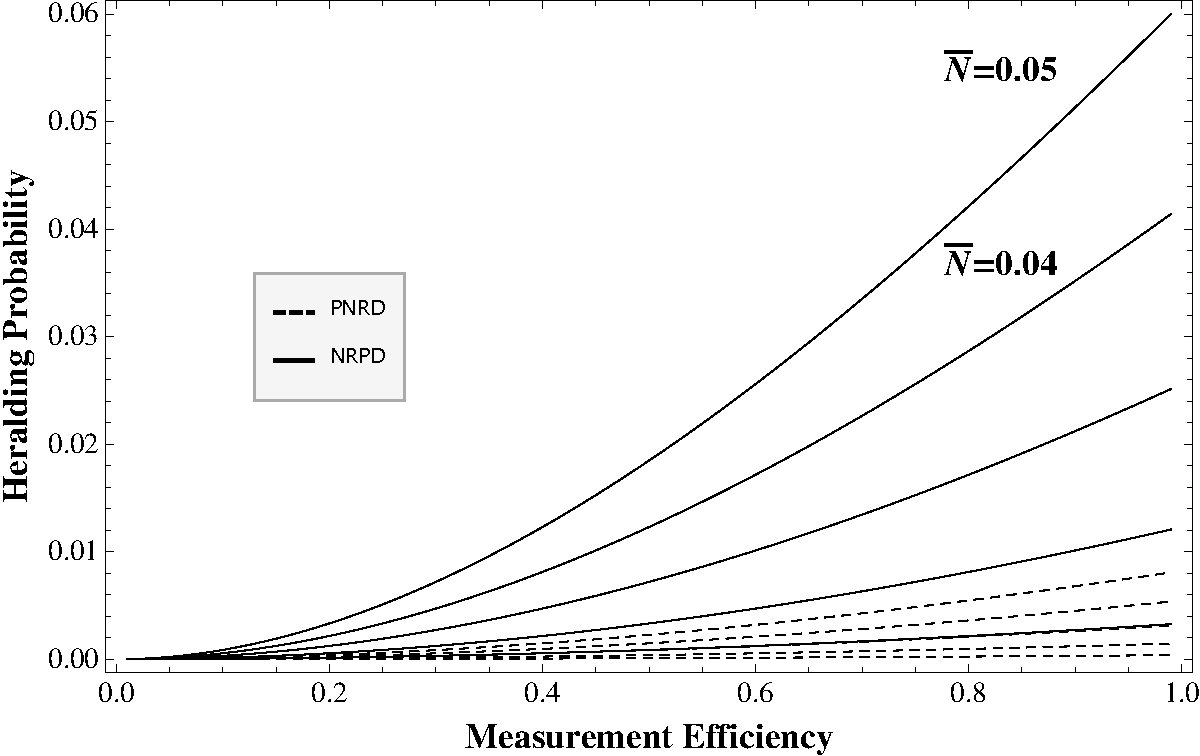
\includegraphics[width=0.47\textwidth]{figures/finalHeraldBothCON.pdf}
    \label{fig:chap3:con:heralding_prob}
    }
    \subfigure[Fidelity of entanglement.]{
    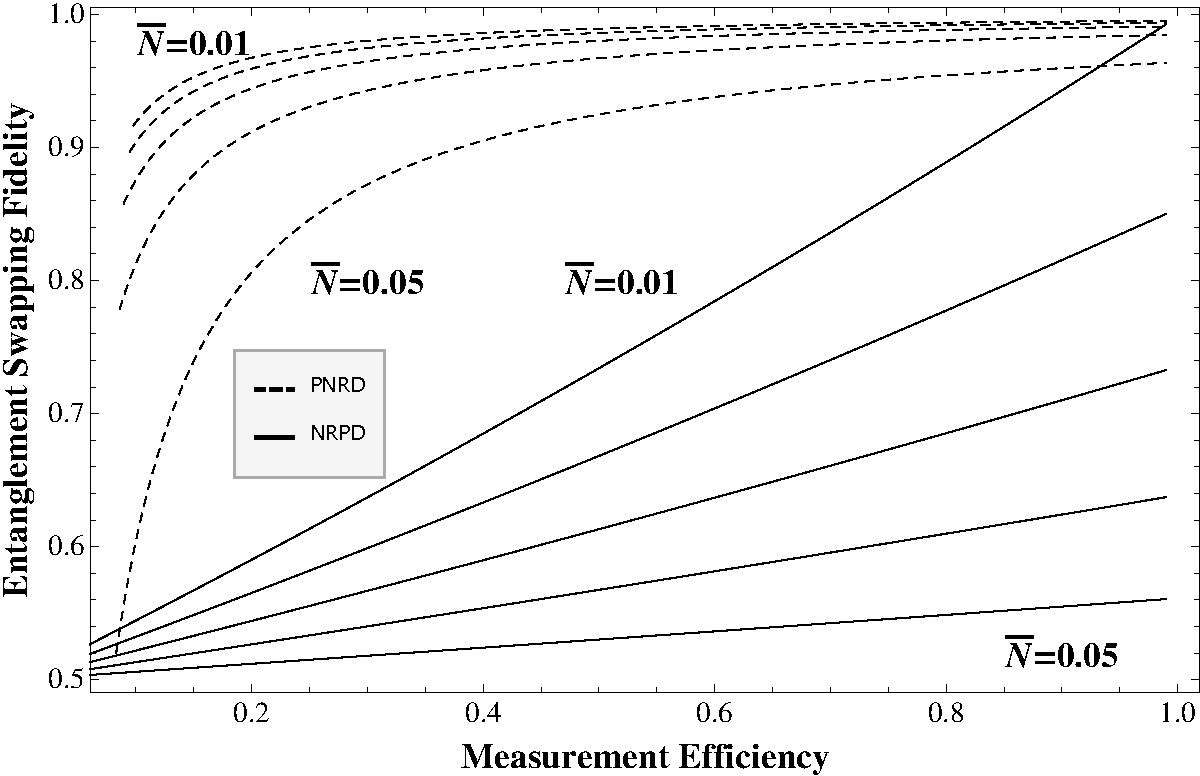
\includegraphics[width=0.47\textwidth]{figures/finalFidelityBothCON.pdf}
    \label{fig:chap3:con:fidelity}
    }
    \subfigure[Fidelity ratio for cross- and co-polarized heralding events.]{
    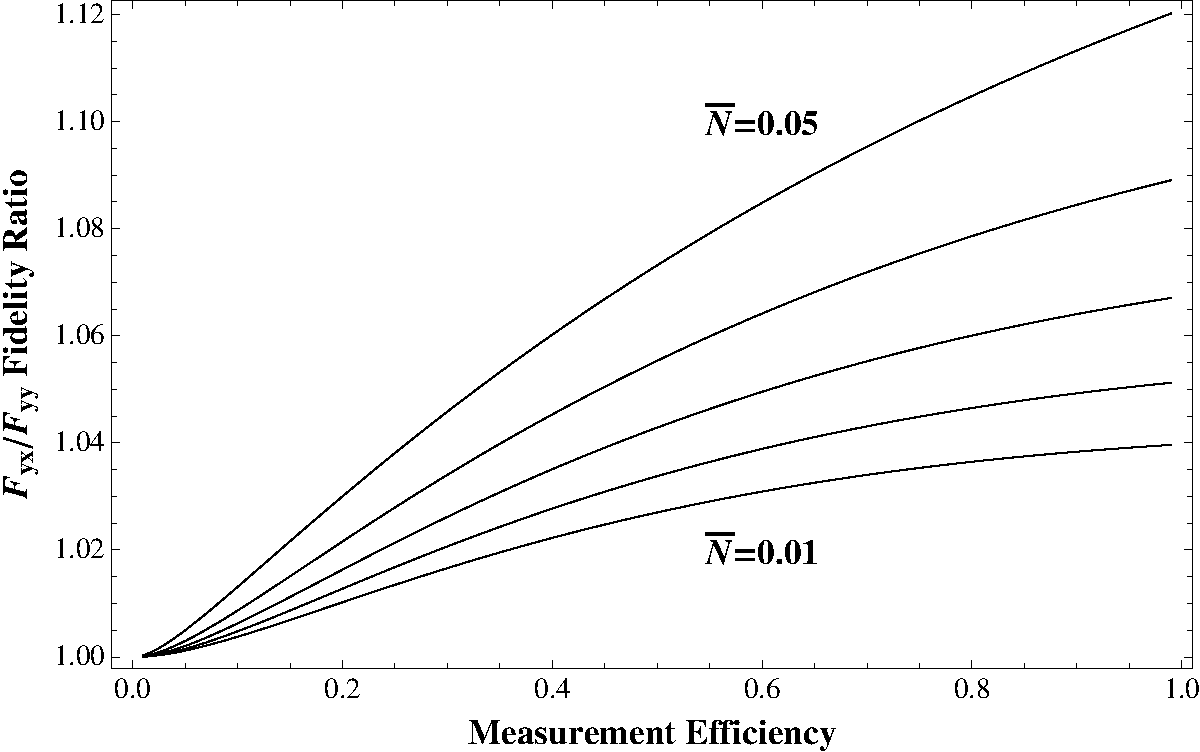
\includegraphics[width=0.47\textwidth]{figures/ratioplot.pdf}
    \label{fig:chap3:con:ratio}
    }
	%\input{spdc_dlcz_fin.pdf_t}
	\caption{Figures of merit for Gaussian state entanglement connection (PNRD and NRPD) for $\bar{N}=0.01-0.05~\pna{\Delta N=0.01}$. 
	\label{fig:merit:entanglement_connection}}
\end{figure}

We will first consider the particular case of a $\mathbf{y}-$polarized click at
$D_A$ and a $\mathbf{x}-$polarized click at $D_B$, and then extrapolate to
other possibilities: a $\mathbf{x}-$polarized click at $D_A$ and a
$\mathbf{y}-$polarized click at $D_B$, and co-polarized clicks at both $D_A$
and $D_B$. Applying these trace identities in a PNRD scheme, the
post-measurement state of the ensembles is
\begin{align}
\hat{\rho}_{\textrm{post}}^{yx}& =
\frac{1}{P_{\textrm{herald}}^{yx}}\int 
\prod_{i=x,y}
\frac{d^2 \zeta_{I_i^A}}{\pi^2} 
\frac{d^2 \zeta_{I_i^B}}{\pi^2} 
D_N\pna{\hat{S}_{I_i^A},\zeta_{I_i^A}} 
D_N\pna{\hat{S}_{I_i^B},\zeta_{I_i^B}}  \nonumber \\
& \qquad \cdot \int 
\frac{d^2 \zeta_{S_y^A}}{\pi^2} 
\frac{d^2 \zeta_{S_x^B}}{\pi^2}
\chi_A^{\rho_{\textrm{out}}}\pna{\bm{\zeta}} 
\pna{1-|\zeta_{S_y^A}|^2}\pna{1-|\zeta_{S_x^B}|^2},
\end{align}
where the heralding probability is
\eqn{
P_{\textrm{herald}}^{yx} =
\int 
\frac{d^2 \zeta_{S_y^A}}{\pi^2} 
\frac{d^2 \zeta_{S_x^B}}{\pi^2}
\chi_A^{\rho_{\textrm{out}}}\pna{\pnb{\zeta_{S_y^A},\zeta_{S_y^B},\zeta_{S_x^A},\zeta_{S_x^B},0,0,0,0}^T} 
\pna{1-|\zeta_{S_y^A}|^2}\pna{1-|\zeta_{S_x^B}|^2}.
}
Applying the Gaussian moment factoring theorem, this heralding probability is
\begin{align}
P_{\textrm{herald}}^{yx}&=\frac{1}{D_2}\langle \pna{1-|\zeta_{S_y^A}|^2}\pna{1-|\zeta_{S_x^B}|^2} \rangle \nonumber \\
	&=\frac{1}{D_2^3}\pnb{D_2^2-2\pna{1+\eta_{\textrm{meas}}\bar{N}}D_2+\pna{1+\eta_{\textrm{meas}}\bar{N}}^2} \nonumber \\
	& = \frac{\eta^2_{\textrm{meas}} \bar{N}^2 (\eta_{\textrm{meas}}  \bar{N} (\eta_{\textrm{meas}}  \bar{N}+3)+3)^2}{(\eta_{\textrm{meas}}  \bar{N}+1)^{10}},
\end{align}
where $\langle~~\rangle$ denotes ensemble averaging treating $\bm{\zeta}$ as a
complex-valued Gaussian random vector whose probability density function is a
marginal distribution of Eqn.~\ref{eq:chap3:moments}, with
$D_2=\pna{1+\eta_{\textrm{meas}}\bar{N}}^4$. Note that the second-moments of
the signal modes reaching the photodetectors are all identical, so the
heralding probabilities for each of the four heralding probabilities mentioned
earlier are equal. Therefore, $P_{\textrm{herald}}=4P_{\textrm{herald}}^{yx}$
for the PNRD case. Applying the trace identities in
Eqn~\ref{eq:chap3:trace_id}, the post-measurement joint density operator for
the NRPD scheme is
\begin{align}
\hat{\rho}_{\textrm{post}}^{yx}& =
\frac{1}{P_{\textrm{herald}}^{yx}}\int \prod_{i=x,y}
\frac{d^2 \zeta_{I_i^A}}{\pi^2} 
\frac{d^2 \zeta_{I_i^B}}{\pi^2} 
D_N\pna{\hat{S}_{I_i^A},\zeta_{I_i^A}} 
D_N\pna{\hat{S}_{I_i^B},\zeta_{I_i^B}}  \nonumber \\
& \qquad \cdot \int 
\frac{d^2 \zeta_{S_y^A}}{\pi^2} 
\frac{d^2 \zeta_{S_x^B}}{\pi^2}
\chi_A^{\rho_{\textrm{out}}}\pna{\bm{\zeta}} 
\pnb{\pi\delta\pna{\zeta_{S_y^A}}-1}\pnb{\pi\delta\pna{\zeta_{S_x^B}}-1}.
\end{align}
Tracing out the idler excitation modes, the NRPD heralding probability is 
\begin{align}
& P_{\textrm{herald}}^{yx} = \nonumber \\
& \qquad \int 
\prod_{i=x,y}
\frac{d^2 \zeta_{S_i^A}}{\pi^2} 
\frac{d^2 \zeta_{S_i^B}}{\pi^2} \chi_A^{\rho_{\textrm{out}}}\pna{\pnb{\zeta_{S_y^A},\zeta_{S_y^B},\zeta_{S_x^A},\zeta_{S_x^B},0,0,0,0}^T} 
\pnb{\pi\delta\pna{\zeta_{S_y^A}}-1}\pnb{\pi\delta\pna{\zeta_{S_x^B}}-1},
\end{align}
which yields
\eqn{
P_{\textrm{herald}}^{yx} = \frac{\eta ^2_{\textrm{meas}} \bar{N}^2}{(\eta_{\textrm{meas}}  \bar{N}+1)^4}.
}
This PNRD heralding probability and PNRD fidelity, as well as the NRPD
heralding probability and fidelity are shown in
Fig.~\ref{fig:merit:entanglement_connection}. The results for heralding
probability are consistent with our understanding of multiple-excitation
effects, as described previously in the context of entanglement distribution in
Section~\ref{sec:numerics}: reading from ensembles with a higher average spin
excitation $\bar{N}$ will yield more anti-Stokes photons, resulting in a higher
likelihood of a heralding event when the photodetectors cannot resolve photon
number.

The fidelity, when a $\mathbf{y}$-polarized $D_A$ click and a
$\mathbf{x}$-polarized $D_B$ click provide the herald, is given by
\begin{align}
F_{yx} & = \bra{\psi_{1}} \hat{\rho}_{\textrm{post}}^{yx} \ket{\psi_1} \nonumber \\
& =\frac{1}{P_{\textrm{herald}}^{yx}}\int 
\prod_{i=x,y}\frac{d^2 \zeta_{I_i^A}}{\pi^2} 
\frac{d^2 \zeta_{I_i^B}}{\pi^2} 
\pnb{1-\frac{|\zeta_{I_x^A}\zeta_{I_y^B}-\zeta_{I_y^A}\zeta_{I_x^B}|^2}{2}}  \nonumber \\
& \qquad \cdot \int 
\frac{d^2 \zeta_{S_y^A}}{\pi^2} 
\frac{d^2 \zeta_{S_x^B}}{\pi^2}
\chi_A^{\rho_{\textrm{out}}}\pna{\bm{\zeta}} 
\pna{1-|\zeta_{S_y^A}|^2}\pna{1-|\zeta_{S_x^B}|^2} \nonumber \\
& = \frac{1}{D_1 P_{\textrm{herald}}^{yx}}\langle \pna{1-|\zeta_{S_y^A}|^2}\pna{1-|\zeta_{S_x^B}|^2}\pna{1-\frac{|\zeta_{I_x^A}\zeta_{I_y^B}-\zeta_{I_y^A}\zeta_{I_x^B}|^2}{2}}  \rangle.
\end{align}

The necessary higher-order moments for this calculation are, from Gaussian moment factoring
\begin{align}
 \langle |\zeta_{I_x^A}\zeta_{I_y^B}-\zeta_{I_y^A}\zeta_{I_x^B}|^2 \rangle & = \langle |\zeta_{I_x^A}|^2 \rangle \langle |\zeta_{I_y^B}|^2 \rangle+\langle |\zeta_{I_y^A}|^2 \rangle \langle |\zeta_{I_x^B}|^2\rangle \nonumber \\
 \langle |\zeta_{S_y^A}|^2  |\zeta_{I_x^A}\zeta_{I_y^B}-\zeta_{I_y^A}\zeta_{I_x^B}|^2 \rangle & = \langle |\zeta_{S_y^A}|^2\rangle \langle |\zeta_{I_x^A}|^2\rangle \langle |\zeta_{I_y^B}|^2\rangle + \langle |\zeta_{S_y^A}|^2\rangle \langle |\zeta_{I_y^A}|^2\rangle \langle |\zeta_{I_x^B}|^2\rangle \nonumber \\
 & \qquad + |\langle \zeta_{S_y^A} \zeta_{I_x^A}\rangle|^2 \langle | \zeta_{I_y^B} |^2\rangle + |\langle \zeta_{S_y^A} \zeta_{I_x^B} \rangle|^2 \langle | \zeta_{I_y^A}  |^2\rangle \nonumber \\
 \langle |\zeta_{S_x^B}|^2 |\zeta_{I_x^A}\zeta_{I_y^B}-\zeta_{I_y^A}\zeta_{I_x^B}|^2 \rangle & = \langle |\zeta_{S_x^B}|^2\rangle \langle |\zeta_{I_x^A}|^2\rangle \langle |\zeta_{I_y^B}|^2\rangle + \langle |\zeta_{S_x^B}|^2\rangle \langle |\zeta_{I_y^A}|^2\rangle \langle |\zeta_{I_x^B}|^2\rangle \nonumber \\
  & \qquad + |\langle \zeta_{S_x^B} \zeta_{I_y^B}\rangle|^2 \langle | \zeta_{I_x^A} |^2\rangle + |\langle \zeta_{S_x^B} \zeta_{I_y^A} \rangle|^2 \langle | \zeta_{I_x^B}  |^2\rangle \nonumber \\
 \langle |\zeta_{S_y^A}|^2  |\zeta_{S_x^B}|^2 |\zeta_{I_x^A}\zeta_{I_y^B}-\zeta_{I_y^A}\zeta_{I_x^B}|^2 \rangle  & = \langle |\zeta_{S_y^A}|^2\rangle \langle |\zeta_{S_x^B}|^2\rangle \langle |\zeta_{I_x^A}|^2\rangle \langle |\zeta_{I_y^B}|^2\rangle \nonumber \\
 & + \langle |\zeta_{S_y^A}|^2\rangle \langle |\zeta_{S_x^B}|^2\rangle \langle |\zeta_{I_y^A}|^2\rangle \langle |\zeta_{I_x^B}|^2\rangle \nonumber \\
   &  + |\langle \zeta_{S_y^A} \zeta_{I_x^A}\rangle|^2 |\langle \zeta_{S_x^B} \zeta_{I_y^B}\rangle|^2+ |\langle \zeta_{S_y^A} \zeta_{I_x^B} \rangle|^2 |\langle \zeta_{S_x^B} \zeta_{I_y^A} \rangle|^2  \nonumber \\
   &  + |\langle \zeta_{S_y^B} \zeta_{I_x^A}\rangle|^2 \langle| \zeta_{S_x^B}|^2\rangle \langle|\zeta_{I_y^B}|^2\rangle + |\langle \zeta_{S_y^A} \zeta_{I_x^B}\rangle|^2 \langle| \zeta_{S_x^B}|^2\rangle \langle|\zeta_{I_y^B}|^2\rangle  \nonumber \\
     &  + |\langle \zeta_{S_x^B} \zeta_{I_y^B}\rangle|^2 \langle| \zeta_{I_x^A}|^2\rangle \langle|\zeta_{S_y^A}|^2\rangle + |\langle \zeta_{S_x^B} \zeta_{I_y^A}\rangle|^2 \langle| \zeta_{S_y^A}|^2\rangle \langle|\zeta_{I_x^B}|^2\rangle \nonumber \\
     &-\left[\langle \zeta_{S_y^A} \zeta_{I_x^A}\rangle \langle \zeta_{S_y^{A}}^* \zeta_{I_x^{B}}^*\rangle \langle \zeta_{S_x^B} \zeta_{I_y^B}\rangle \langle \zeta_{S_x^{B}}^* \zeta_{I_y^{A}}^*\rangle \right.\nonumber \\
     & \left.\qquad\qquad + \langle \zeta_{S_y^A} \zeta_{I_x^B}\rangle \langle \zeta_{S_y^{A}}^* \zeta_{I_x^{A}}^*\rangle \langle \zeta_{S_x^B} \zeta_{I_y^A}\rangle \langle \zeta_{S_x^{B}}^* \zeta_{I_y^{B}}^*\rangle\right]
     \label{eq:yx:moment}
\end{align}
Applying the covariance matrix in Eqn.~\ref{eq:chap3:moments} to these
higher-order moment expressions, the PNRD fidelity is given by
\begin{align}
F_{yx}&=\left[\frac{1}{D_1^3}\pnb{D_1^2-2\pna{1+\eta_{\textrm{meas}}\bar{N}}1_2+\pna{1+\eta_{\textrm{meas}}\bar{N}}^2}\right.\nonumber\\
& \qquad \left.-\frac{1}{2D_1} \left(\frac{2\pna{1+\bar{N}}^2}{D_1^2}-\frac{4\pna{1+\eta_{\textrm{meas}}\bar{N}}\pna{1+\bar{N}}^2+8\eta\pna{1+\bar{N}}\tilde{N}^2}{D_1^3}\right.\right.\nonumber\\
& \qquad \left.\left.+\frac{2\pna{1+\eta_{\textrm{meas}}\bar{N}}^2\pna{1+\bar{N}}^2 +8 \eta \tilde{N}^2 \pna{1 + \eta_{\textrm{meas}} \bar{N}} \pna{1 + \bar{N}}}{D_1^4}\right)\right].
\end{align}
The $F_{xy}$ fidelity is easily seen to be the same as the $F_{yx}$ fidelity,
as in the heralding probability calculation presented earlier. While the
$F_{xx}$ and $F_{yy}$ fidelities will also equal, they will differ from the
cross-polarized fidelities. To find $F_{yy}$, we need to evaluate
\begin{align}
F_{yy} & = \frac{1}{D_1 P_{\textrm{herald}}^{yy}}\langle
\pna{1-|\zeta_{S_y^A}|^2}\pna{1-|\zeta_{S_y^B}|^2}\nonumber \\ & \qquad \cdot\pna{1-\frac{|\zeta_{I_x^A}\zeta_{I_y^B}-\zeta_{I_y^A}\zeta_{I_x^B}|^2}{2}}  \rangle.
\end{align}
The calculation is identical to that for $F_{yx}$ save for the eighth-order
moment, which factors into
\begin{align}
& \langle |\zeta_{S_y^A}|^2  |\zeta_{S_y^B}|^2|\zeta_{I_x^A}\zeta_{I_y^B}-\zeta_{I_y^A}\zeta_{I_x^B}|^2 \rangle = \nonumber \\
& \qquad\langle |\zeta_{S_y^A}|^2\rangle \langle |\zeta_{S_y^B}|^2\rangle \langle |\zeta_{I_x^A}|^2\rangle \langle |\zeta_{I_y^B}|^2\rangle + \langle |\zeta_{S_y^A}|^2\rangle \langle |\zeta_{S_y^B}|^2\rangle \langle |\zeta_{I_y^A}|^2\rangle \langle |\zeta_{I_x^B}|^2\rangle \nonumber \\
       & \qquad\qquad + |\langle \zeta_{S_y^B} \zeta_{I_x^A}\rangle|^2 \langle| \zeta_{S_y^A}|^2\rangle \langle|\zeta_{I_y^B}|^2\rangle + |\langle \zeta_{S_y^A} \zeta_{I_x^A}\rangle|^2 \langle| \zeta_{S_y^B}|^2\rangle \langle|\zeta_{I_y^B}|^2\rangle  \nonumber \\
       & \qquad\qquad + |\langle \zeta_{S_y^A} \zeta_{I_x^B}\rangle|^2 \langle| \zeta_{I_y^A}|^2\rangle \langle|\zeta_{S_y^B}|^2\rangle + |\langle \zeta_{S_y^B} \zeta_{I_x^B}\rangle|^2 \langle| \zeta_{S_y^A}|^2\rangle \langle|\zeta_{I_y^A}|^2\rangle.\label{eq:yy:moment}
\end{align}

Comparing Eqn.~\ref{eq:yy:moment} and~\ref{eq:yx:moment}, it immediately
becomes obvious that the $F_{yy}$ and $F_{yx}$ differ in their contribution to
the overall entanglement fidelity. Prior to our Gaussian state analysis, we
assumed that ensembles A and B had loaded pure singlet states prior to
entanglement swapping. Their pure singlet states yield a perfect fidelity in
both NRPD and PNRD photodetection schemes with the heralding of cross-polarized
photons at detectors $D_A$ and $D_B$. However, the measurement of co-polarized
photons is indistinguishable from a cross-polarized photon measurement, even
though entanglement need not be successfully swapped when the herald comes from
co-polarized photons. As such, we define the fidelity of entanglement as
\eqn{
F_E = \frac{P_{\textrm{success}}}{P_{\textrm{herald}}}=  \frac{2P_{\textrm{herald}}^{yx}F_{yx}+2P_{\textrm{herald}}^{yy}F_{yy}}{P_{\textrm{herald}}}.
}
Figs.~\ref{fig:chap3:con:fidelity} and~\ref{fig:chap3:con:ratio} show the
fidelity of entanglement following a swapping operation. As in polarization
entanglement distribution, reading and producing multiple-excitations increases
heralding probability at the expense of the entanglement fidelity. In this
regard, the fidelity plots for emphasize some significant differences between
the PNRD and NRPD cases. From the post-measurement density operator, this NRPD
fidelity is given by
\begin{align}
F_{yx} & = \bra{\psi_{1}} \hat{\rho}_{\textrm{post}}^{yx} \ket{\psi_1} \nonumber \\
& =\frac{1}{P_{\textrm{herald}}^{yx}}\int 
\prod_{i=x,y}
\frac{d^2 \zeta_{I_i^A}}{\pi^2} 
\frac{d^2 \zeta_{I_i^B}}{\pi^2} 
\pnb{1-\frac{|\zeta_{I_x^A}\zeta_{I_y^B}-\zeta_{I_y^A}\zeta_{I_x^B}|^2}{2}}  \nonumber \\
& \qquad \cdot \int 
\frac{d^2 \zeta_{S_y^A}}{\pi^2} 
\frac{d^2 \zeta_{S_x^B}}{\pi^2}
\chi_A^{\rho_{\textrm{out}}}\pna{\bm{\zeta}} 
\pnb{\pi\delta\pna{\zeta_{S_y^A}}-1}\pnb{\pi\delta\pna{\zeta_{S_x^B}}-1}.\label{eqn:fyx_nrpd}
\end{align}
Unlike the difference in moment factoring present in the PNRD fidelity
calculation, the NRPD fidelity is identical for to cross-polarized and
co-polarized photodetection events, as is evident from the NRPD POVM applied in
Eqn.~\ref{eqn:fyx_nrpd}. This calculation is only dependent on the
second-moments of the idler ensembles and the normalizations inherent in the
marginal probability distributions following photodetection, each of which is
independent of photon polarization. Equation~\ref{eqn:fyx_nrpd} thus simplifies
to
\begin{align}
    F_{yx}=\frac{1}{P_{\textrm{herald}}^{yx}}\pnb{\frac{(\bar{N}+1)^6 (\eta_{\textrm{meas}}  \bar{N}+1)^7-2 (\bar{N}+1)^6 (\eta_{\textrm{meas}}  \bar{N}+1)^6+1}{(\bar{N}+1)^{10} (\eta_{\textrm{meas}}  \bar{N}+1)^9} +\frac{1}{D_1}-\frac{\pna{\bar{N}+1}^2}{D_1^3}},
\end{align}
which is plotted in Fig.~\ref{fig:chap3:con:fidelity}. The PNRD case lets us
actively discard garbage photodetection events that might result from
multiple-excitations present at entanglement distribution. In this case, we
know that having matching, \emph{single} counts at $D_A$ and $D_B$ will very
likely correspond to a successful entanglement swapping operation with
photon-number resolving detectors. On the other hand, high $\bar{N}$, even in
the presence of high measurement efficiency, severely affects our NRPD
entanglement fidelity, because NRPD cannot distinguish false heralding
events. Also surprising is the ratio of the fidelity of entanglement for
cross-polarized and co-polarized photodetection events, as shown in
Fig.~\ref{fig:chap3:con:ratio}. These fidelities are very close to each other,
although they begin to diverge as $\bar{N}$ increases. That they are so close
in value is somewhat surprising because cross-polarized photodetection was
predicted for unity entanglement fidelity in the case of a pure singlet
distribution, whereas co-polarized photodetection would not necessarily be
indicative of a singlet state remaining in the idler ensembles.


\section{Summary and Outlook~\label{chap:conclusion}}

% quantum information perspective and overview
To date, the theoretical progress of quantum information science and
engineering has surpassed its experimental achievements. This thesis paints a
detailed picture of what future long-distance quantum communication networks
might look like, and their limitations. In the course of this work, we have
analyzed quantum networks that distribute polarization entanglement using
neutral atomic ensembles. This analysis focuses on three areas. We first
abstracted quantized light-ensemble interactions within a heralding atomic
memory and determined that these interactions preclude a Gaussian state
analysis of local entanglement distribution (Chapter~\ref{chap:atomic},
Appendix~\ref{chap:appb}). After describing the potential losses in an
entanglement distribution architecture, we applied the $\textrm{SU}\pna{2}$
representation of beam splitter operators to model loss in a number state
basis, and performed a Gaussian state analysis of polarization entanglement
swapping (Chapter~\ref{chap:herald}). A number-state analysis of the
entanglement distribution captures the joint state of the heralding light and
atomic excitations, accounting for imperfections in transmission loss,
photodetection efficiency and counting resolution, and multiple-pair events at
the downconversion source.

% Findings 

The numerical characterization of entanglement distribution and connection
presented in this thesis is so far consistent with our physical intuition of
how such networks should behave. In particular, the probability of a successful
heralding event is independent of whether a single, significant, uniform
efficiency loss is located either before or after an ensemble memory, or during
photodetection. With regards to the probability measuring a single photon, all
losses are effectively the same. The same is not true for fidelity. A uniform
transmission loss between the entanglement source and the ensembles will
significantly reduce the likelihood that you've stored a polarization Bell
state, but significant quantum efficiency losses at photodetection are less
likely to diminish that fidelity. Increasing the pump power at the entanglement
source increases the likelihood of multiple-pair events, increasing the
heralding probability but making the fidelity more sensitive to transmission
and photodetection efficiency losses. These results are true for both
number-resolving and non-resolving photodetectors. For both entanglement
distribution and connection, heralding probabilities for non-resolving
detectors are higher, but the fidelities are significantly lower. Many of these
same issues appear in entanglement swapping as well.

% Extensions

Two areas in this thesis are particularly ripe for extension and exploration:
further investigation into the mechanisms and imperfections of ensemble
memories that distribute polarization entanglement, and formalizing the number
state analysis of systems with loss-modeling beam splitters. Several possible
extensions are relatively straightforward, such as the inclusion of phase
offsets between orthogonally-polarized paths in during entanglement
distribution. Others require a more careful consideration of the underlying
physics of quantum memories. For example, the performance analysis of
polarization entanglement distribution presented in this thesis omits the
presence of spin decoherence in the atomic ensembles. In quantifying the
singlet-storage fidelity, there is a tradeoff between the time scale of
decoherence of Dicke excitations, the time it takes for a single heralding
photon to reach a photodetector, and the post-memory transmission efficiency
(which scales with the post-transmission length). Spin decoherence of the
ensemble may therefore be a significant factor limiting the optimal physical
distance that local entanglement distribution can cover. Another possible
departure would be to discard the DLCZ approach entirely, using a stimulated
Raman or EIT approach, instead of a spontaneous Raman process. The Hamiltonian
in this approach would be amenable to a traditional Gaussian state analysis,
and would allow for deterministic control of read and write processes in
entanglement distribution. As of the writing of this thesis, however, there is
currently no accepted means of nondestructive verification of successful
entanglement distribution in a coherently-controlled $\Lambda$-level atomic
ensemble. This open problem makes certain long-distance quantum communication
tasks, such as repeated entanglement connection, difficult to accomplish using
a driven Raman process.

Unrelated to the question of memories is formalizing the architectural analysis
of loss-modeling beam splitters. The $\textrm{SU}\pna{2}$ number-state
representation for \emph{single} beam splitters is discussed in great detail
by~\cite{PhysRevA.40.1371}. Summation compositions of beam splitter
coefficients determined important architectural figures of merit---heralding
probability, fidelity, and success probability---in the course of this work,
but were calculated numerically. With a number-state basis, what general
properties or figures of merit of a quantum network can we determine if we
limit ourselves to linear optical elements (e.g., 50-50 and polarizing beam
splitters, loss elements), photodetectors, and photon-number conserving
nonlinear optical elements (e.g., heralding quantum memories or Kerr crystals)?
In particular, do any of the properties of a beam splitter coefficient
introduced in Chapter~\ref{chap:herald} permit any useful, analytical
simplifications when using the joint density operator of a network to calculate
a figure of merit? Is a number-state analysis consistent with a SPDC Gaussian
state analysis when nonlinear elements are excluded and we are limited entirely
to the propagation of optical fields? Answers to these questions could possibly
alleviate the exhausting notational and computational difficulties currently
necessitated by number-state analysis.


% Specify following sections are appendices. Use \appendix* if there
% only one appendix.
%\appendix
%\section{}

% If you have acknowledgments, this puts in the proper section head.

\begin{acknowledgments}

  We thank F. Wong, V. Vuletic, Z. Dutton, S. Johnson, R. Nair, and B. J. Yen
  for useful discussions and advice. This work was supported by the DARPA
  Quantum Entanglement Science and Technology (QuEST) program.

\end{acknowledgments}

% Create the reference section using BibTeX:
\bibliography{citations/proposal}

\end{document}
%
% ****** End of file apstemplate.tex ******

